\documentclass[conference,9pt]{IEEEtran}
\usepackage{xcolor}
\usepackage{cite}
\usepackage{epsfig}
\usepackage{amssymb}
\usepackage{amsmath}
\usepackage{graphicx}
\graphicspath{ {./} }

\begin{document}
\title{Practical 2a}

\author{
\IEEEauthorblockN{Albert Acebron}
\IEEEauthorblockA{NIU: 1458626}
}


% make the title area
\maketitle
\begin{abstract}
This practical will be based on applying ML to received signals
\end{abstract}



%----------------------------------------------------------------
% SECTION #1 
\section{Introduction}

\section{Questions}

\subsection{Question 1}
In (1.2) a scalar value is used because the function only represents a single probability distribution (one dimension), but on (1.3) we are multiplying the pdfs of multiple probability distributions, and each one of which has a different mean, so we must use a vector that contains all of these.

In other words, $\mu_x$ on (1.2) is the mean of the gaussian distribution at hand, whereas $\mu_x$ on (1.3) is a vector that contains the means of the probability distributions of the signal at different times ($n=0,1,...$).

This can be proved by simply taking the expression on (1.2) and multiplying it by other versions of it with different $\mu_x$ values. The result of this multiplication will yield the expression on (1.3) where $\mu_x$ is a vector that contains the different $\mu_x$ mentioned before.
\subsection{Question 2}
Given that we know that 
$$\mu_x(n)=mean(x(n))=mean(Acos(2\pi f_dn+\phi)+w(n))$$

and $mean(w(n))=0\forall n$ because of their definition as representation of a distribution of mean 0, so:
$$\mu_x(n)=mean(Acos(2\pi f_dn+\phi))$$

Which is a constant, thus:
$$\mu_x(n)=Acos(2\pi f_dn+\phi)$$

And given that the multi-dimensional pdf of $x$ will be a multiplication of gaussian pdfs (since each $x(n)$ has a gaussian pdf), which is the expression provided in (1.3), we can derive that the multi-dimensional pdf that we are searching for will have the shape of (1.3) with $$\mu_x(n)=Acos(2\pi f_dn+\phi)$$.

\subsection{Question 3}
Given that $N=1$ we will only deal with a single pdf, and following the discussion provided on question 2 we can ascertain that the pdf of $x(0)$ will be a gaussian\footnote{This is because the pdf would be the result of multiplying 1 guassians, thus a single guassian} with mean $\mu = Acos(2\pi f_d 0+\phi)=Acos(\phi)$ and standard deviation $\sigma=1$.

Therefore, we can directly graph these functions by computing their values:

\begin{verbatim}
  x = -10:0.1:10;
  sigma = 1;
  hold on;
  mu = 5*cos(pi/4);
  y = (1/(sigma*sqrt(2*pi)))
    .*exp(-((x-mu).^2)/(2*sigma^2));
  plot(x,y)
  mu = 5*cos(pi/2);
  y = (1/(sigma*sqrt(2*pi)))
    .*exp(-((x-mu).^2)/(2*sigma^2));
  plot(x,y)
  mu = 5*cos(3*pi/4);
  y = (1/(sigma*sqrt(2*pi)))
    .*exp(-((x-mu).^2)/(2*sigma^2));
  plot(x,y)
\end{verbatim}
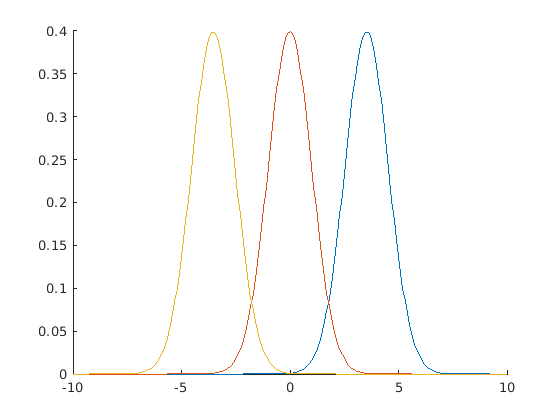
\includegraphics[scale=0.6]{3}

\subsection{Question 4}

\begin{verbatim}
  r=RxSignal(:,1);
  d=500;
  [h, x]=hist(r,d);
  lr=length(r);
  lh=x(end)-x(1)
  plot(x,h.*(d/(lr*lh)));
\end{verbatim}
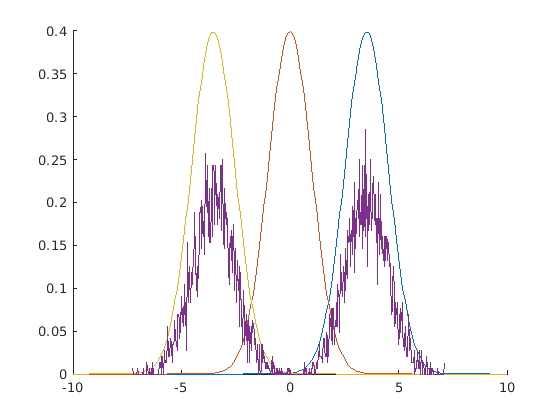
\includegraphics[scale=0.6]{4}

\subsection{Question 5}
We are taking samples in the space domain because we want all the samples to belong to the same pdf for easy matching. If we took the samples at different times each sample would have a different pdf associated with them and thus the method we applied here wouldn't work.

To be able to treat space and time indistictly as domains, the pdfs of the values at different times would need to be the same.
\subsection{Question 6}

\subsection{Question 7}


\section{Conclusion}
We managed to obtain a good estimate of the signal's phase, thus accomplishing our objectives.


\end{document}


